% version 1.01, date 07/03/16, auteur Matthieu Martins-Baltar
\documentclass[compress,xcolor=dvipsnames]{beamer}

%Pour les schémas d'architecture
\usepackage{etex}
\usepackage{tikz}
\usetikzlibrary{shapes,arrows,chains,backgrounds,fit}
%FIN Pour les shémas d'architecture

\usepackage[french]{babel}
\selectlanguage{french}
\usepackage[utf8]{inputenc}
\usepackage[T1]{fontenc}
\usepackage{tikz}
\usepackage{wrapfig}
\usepackage{multirow}
\usepackage{pgfplots}
\usepackage{pdfpages}
\usepackage{vocabulaireUnipikPresentation}
\usepackage{commun/vocabulaireCommun}
\usepackage{hyperref}
\usepackage{movie15}
\usepackage{xcolor}
\usepackage{lscape}
\usepackage{booktabs}
\usepackage{multirow}
\usepackage{colortbl}

\newcommand{\tabincell}[2]{\begin{tabular}{@{}#1@{}}#2\end{tabular}}

\usetheme{Berlin}%{Madrid}

 
 
%Information to be included in the title page:
\title{Débriefing \RQ}
\date{\today}
\author{Pierre Porche}
\institute{\insa}

\setbeameroption{show notes}

 
\begin{document}


\begin{frame}[plain]
	\titlepage
\end{frame}

\begin{frame}{Sommaire}
	\tableofcontents[hideallsubsections]
\end{frame}


\section{Gestion interne et audit}
\subsection{Gestion interne de la qualité}
\begin{frame}
\frametitle{Gestion interne de la qualité}
\begin{itemize}
\item Utilisation de PGPIC
\item Techniques de gestion de la Qualité en évolution permanente
\item Respect du principe de l'amélioration continue
\item Implication globale de l'équipe
\end{itemize}
\end{frame}


\subsection{Résultats de l'audit interne}
\begin{frame}
\frametitle{Justification des résultats de l'audit interne}
\begin{itemize}
\item Cinq remarques
\item Maîtrise des documents au centre des remarques
\item Planification incomplète
\end{itemize}
\end{frame}
 

\section{Gestion Qualité}
\subsection{Outils utilisés}
\begin{frame}
\frametitle{Outils pour la gestion de la qualité}
\begin{block}{PGPIC}
\begin{itemize}
\item Gestion du temps de travail en salle PIC
\item Gestion des réunions
\item Gestion des comptes rendus
\item Gestion des documents
\item Gestion des Faits Techniques
\end{itemize}
\end{block}
\end{frame}


\subsection{Techniques mises en \oe{}uvre}
\begin{frame}
\frametitle{Techniques pour la gestion de la qualité}
\begin{itemize}
\item Délégation de la Gestion des Configurations
\item Réunions hebdomadaires
\item Tableau de bord
\item Campagne d'affichage
\item Implication de tous les membres
\end{itemize}
\end{frame}


\section{Sensibilisation}
\subsection{Sensibilisation de l’équipe}
\begin{frame}
\frametitle{Sensibiliser un équipe hétérogène}
\begin{itemize}
\item Campagne d'affichage
\item Interrogations fréquentes
\item Attribution de risques et opportunités
\item Participation collective à la rédaction des Documents de qualité
\end{itemize}
\end{frame}


\subsection{Sensibilisation du client}
\begin{frame}
\frametitle{Sensibiliser un client non technique}
\begin{itemize}
\item Réunion de lancement axée sur la Qualité
\item Rappels fréquents
\item Réponses vives aux interrogations
\end{itemize}
\end{frame}


\section{Tableaux de bord}
\subsection{Suivi}
\begin{frame}
\frametitle{Suivi des tableaux de bord}
\begin{center}
			\begin{figure}
				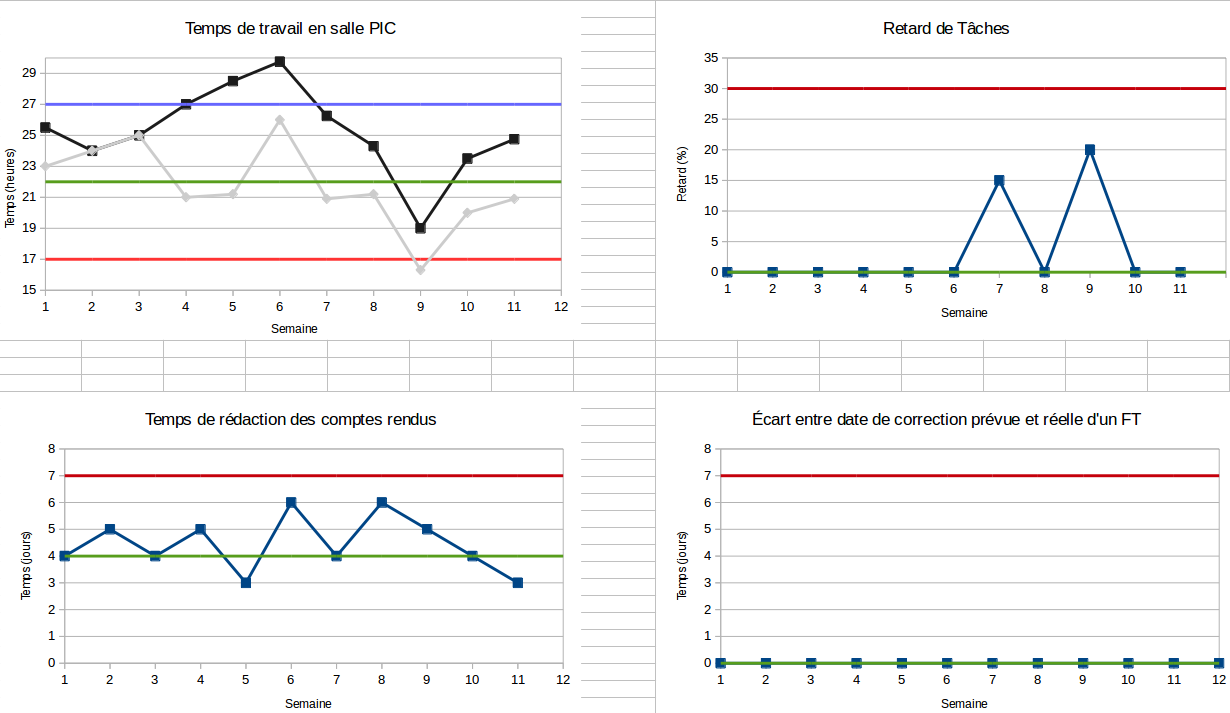
\includegraphics[scale=0.21]{./images/TB.png}
				\caption{Courbes de suivi des indicateurs}
			\end{figure}
		\end{center}
\end{frame}	


\section{Divers}
\begin{frame}
\frametitle{Passation Qualité}
\begin{itemize}
\item Impression 
\item 
\end{itemize}
\end{frame}


\section{Conclusion}
\begin{frame}
\frametitle{Bilan et impressions personnelles}
\begin{itemize}
\item coin
\item coincoin
\end{itemize}
\end{frame}


\end{document}



























